\chapter{Streaming MISRGRU Training Ablations}
\label{app:trnet_modifications}

Before settling on the final streaming MISRGRU configuration reported in
Section~\ref{sec:streaming}, a series of training-level ablations were conducted to identify
the best combination of:
\begin{itemize}
  \item truncated back-propagation-through-time (TBPTT) supervision window
  \item loss function
  \item ConvGRU size
  \item decoder architecture
\end{itemize}
Each ablation isolates one variable while keeping the others fixed.
Results are reported on the same 480-sample test set and evaluated using RSP.

Following parameters were used to train baseline Streaming MISRGRU model:
For TBPTT sequence of 50 frames, chunk size of 16 and loss last N 20.
trained with 2000 samples with 90/10 train/val split. 

Due to time limits of training on DelftBlue cluster all models were given same 
24 hours limit. 


\section*{Truncated BPTT: Loss-last-N}
\label{appsec:lln}

Streaming MISRGRU is trained with TBPTT over sequences of 50 frames.
Computing gradients through the entire sequence is prohibitively expensive, so
back-propagation is truncated to the final $N$ frames.
Loss last N parameter controls both memory cost speed of training and how broadly
the hidden-state trajectory is supervised.

Figure~\ref{fig:lln10vslln35} compares RSP on the evaluation set $N=10$ (where gradients cover only the last 20\% of the sequence) and $N=35$
(covering the last 70\%).

\begin{figure}[h]
  \centering
  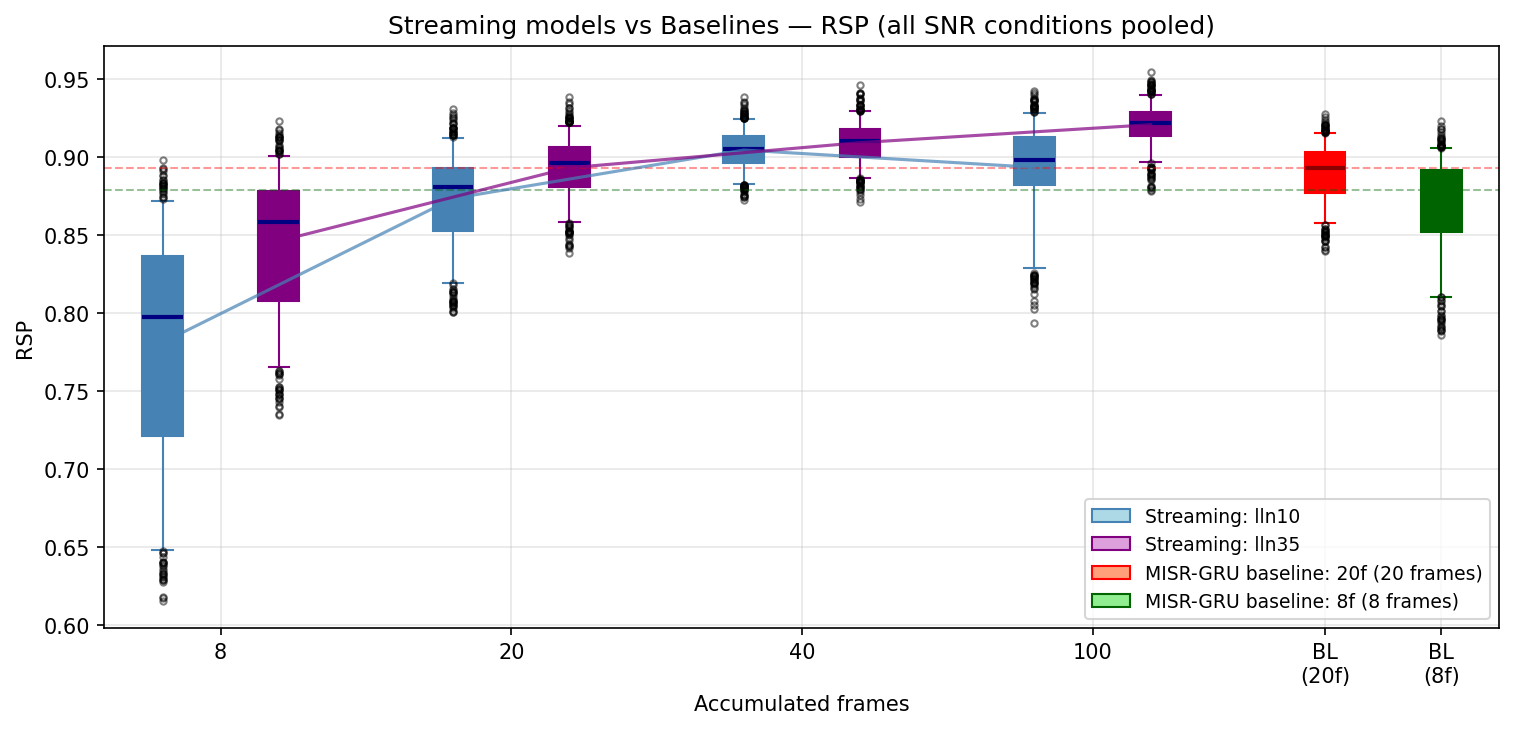
\includegraphics[width=\linewidth]{figures/lln10vslln35.png}
  \caption{RSP evaluation of models when trained with $N=10$ and $N=35$.}
  \label{fig:lln10vslln35}
\end{figure}

\begin{figure}[h]
  \centering
  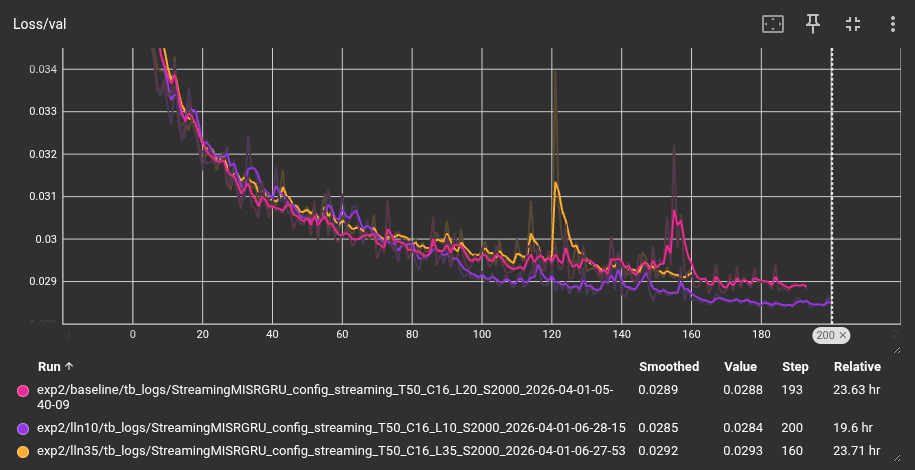
\includegraphics[width=\linewidth]{figures/loss_streaming_lln10_baseline_lln35.png}
  \caption{Loss comparison of baseline streaming model ($N=20$) and models trained with
   $N=10$ and $N=35$.}
  \label{fig:loss_streaming_lln10_baseline_lln35}
\end{figure}

Despite model trained with $N=35$ achieving a highest final L1+Fourier validation loss 
($0.0293$ vs.\ $0.0284$ of $N=10$),
the LLN10 model scores lower on RSP.
The tighter supervision window trains the GRU to produce good outputs at the tail of
the sequence but leaves the early frames weakly regularised.

\section*{Loss function: Fourier vs.\ L1+Fourier}
\label{appsec:loss_streaming}
We trained two streaming models under identical conditions (with lost last N of 20, 
two-GRU 24-channel architecture, deconvolution decoder)
 but with different loss functions:
the pure Fourier loss $\mathcal{L}_\text{Fourier}$ and the combined
$\mathcal{L}_\text{L1+Fourier} = \mathcal{L}_\text{L1} + \lambda\,\mathcal{L}_\text{Fourier}$.
with $\lambda$ being 0.1.

\begin{figure}[h]
  \centering
  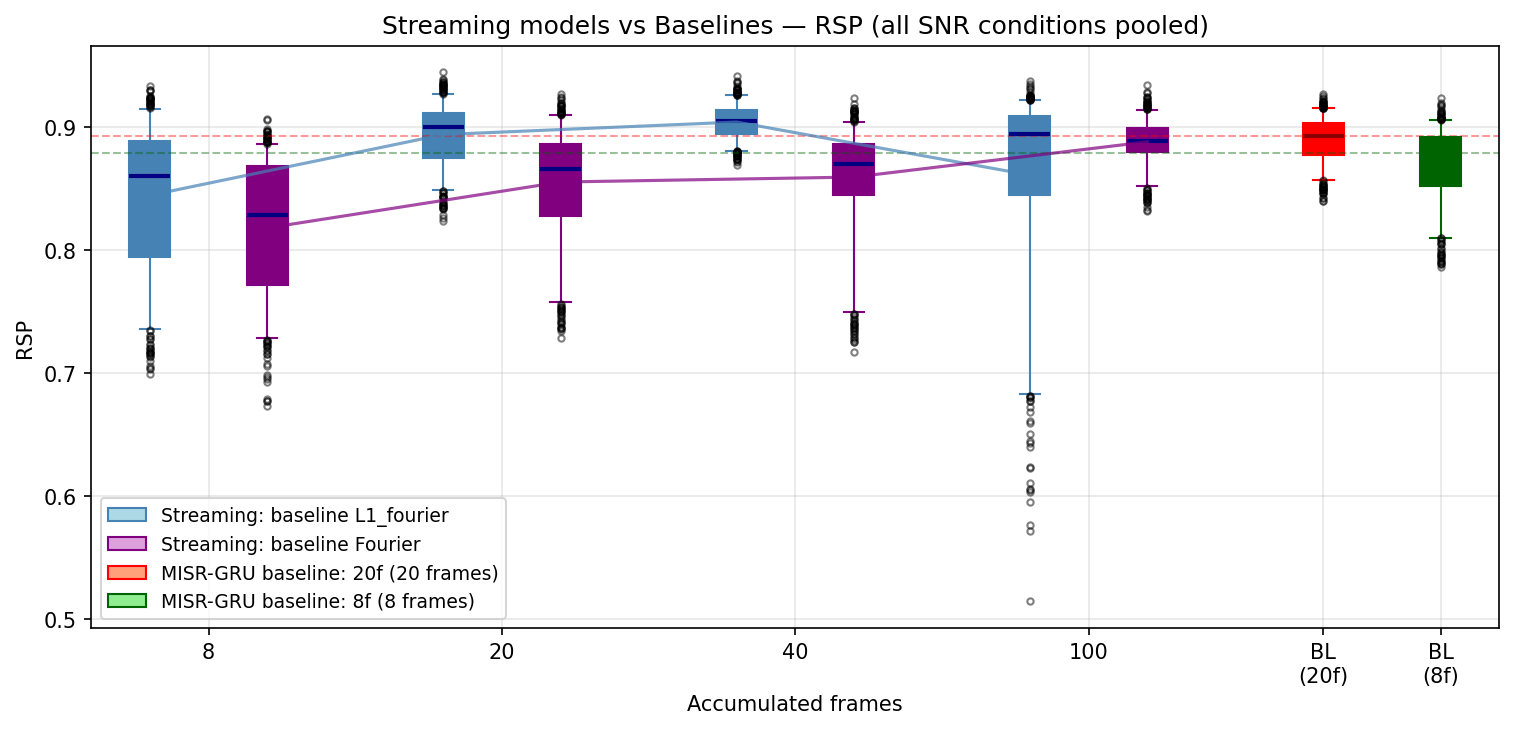
\includegraphics[width=\linewidth]{figures/streaming_l1f_vs_fourier.png}
  \caption{RSP on the test set per SNR condition for streaming MISRGRU trained with
           Fourier-only loss versus combined L1+Fourier loss.}
  \label{fig:streaming_l1f_vs_fourier}
\end{figure}

Figure~\ref{fig:streaming_l1f_vs_fourier} shows that the Fourier-only model outperforms
L1+Fourier, particularly under low-SNR conditions (slow blinking, reduced photon count).
The L1 term introduces a regression-to-mean bias: because SOFI images are dominated by
near-zero background pixels, minimising the mean absolute error encourages the model to
slightly suppress fine structure in order to reduce the background contribution to the loss.
The pure Fourier objective has no such incentive; it rewards spectral fidelity at all
spatial frequencies regardless of pixel intensity.
\textbf{The Fourier-only loss is therefore used for all subsequent streaming experiments.}

\section*{GRU architecture: two 24-channel GRUs vs.\ one 48-channel GRU}
\label{appsec:gru_size}

The original MISRGRU fusion module stacks two ConvGRU layers each with 24 feature channels.
To test whether a single wider GRU with the same total channel budget can match or improve
upon this design, we trained a variant with one ConvGRU of 48 channels.
Both models were trained with the Fourier loss and LLN20.

\begin{figure}[h]
  \centering
  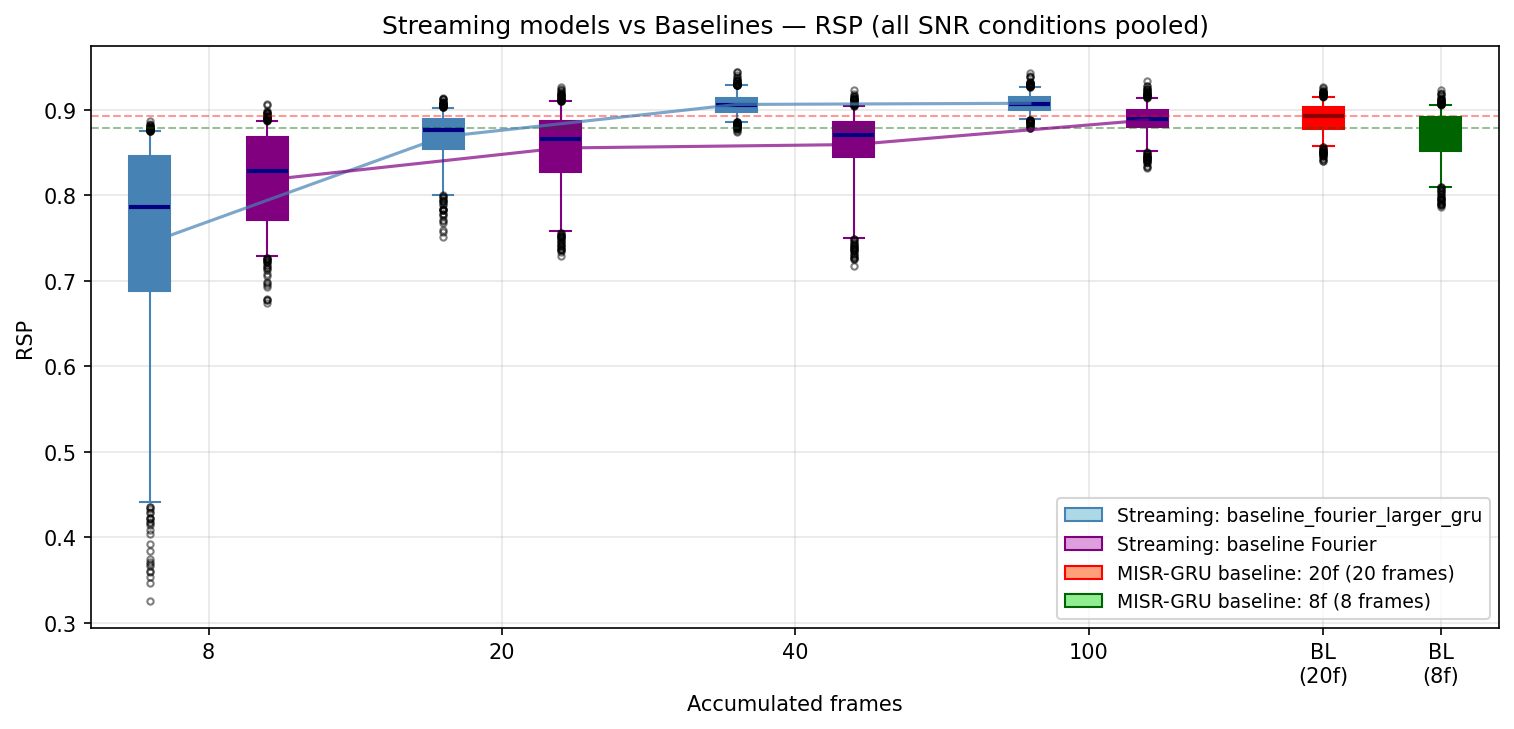
\includegraphics[width=\linewidth]{figures/largergru_vs_fourierbaseline.png}
  \caption{RSP per SNR condition for streaming MISRGRU with two 24-channel ConvGRUs
           versus a single 48-channel ConvGRU, both trained with Fourier loss.}
  \label{fig:largergru_vs_fourierbaseline}
\end{figure}

\begin{figure}[h]
  \centering
  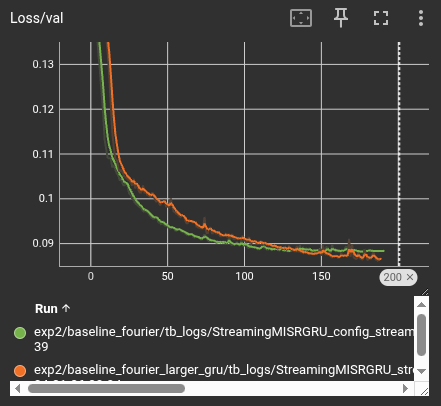
\includegraphics[width=\linewidth]{figures/loss_streaming_architecture_size.png}
  \caption{Validation loss during training of 1x48 ConvGRU vs 2x24 ConvGRUs}
  \label{fig:loss_streaming_architecture_size}
\end{figure}

Figure~\ref{fig:largergru_vs_fourierbaseline} shows that the single 48-channel
configuration ultimately outperforms the two 24-channel baseline on RSP, despite
exhibiting slower convergence during training.
As visible in Figure~\ref{fig:loss_streaming_architecture_size}, the 1$\times$48 model
takes more epochs to reach its lowest validation loss compared to the 2$\times$24 baseline,
yet it achieves a lower final loss and a higher RSP at the end of the 24-hour training limit.

The slower convergence is expected: a single GRU with 48 channels must simultaneously
learn to extract local spatial features and integrate them into a global hidden state.
However, at the end of 24 hour training limit the larger hidden state of the 1$\times$48 GRU provides richer
representational capacity. 
Because the streaming model processes frames one at a time and must maintain all
accumulated information in a single hidden state vector, a wider hidden state can retain
more independent blinking-event statistics simultaneously.

\section*{Decoder: PixelShuffle vs.\ transposed convolution}
\label{appsec:decoder_streaming}

The non-integer SOFI upscaling factor $(2H-7)\times(2W-7)$ requires a decoder that can
produce an output of exact size without cropping artefacts at the boundary.
Two designs were evaluated: a $2\times$ PixelShuffle followed by a centre-crop to discard
the seven-pixel border, and a learned transposed convolution
(\texttt{ConvTranspose2d}) configured to output exactly $(2H-7)\times(2W-7)$ pixels
by adjusting stride, padding, and output-padding.

\begin{figure}[h]
  \centering
  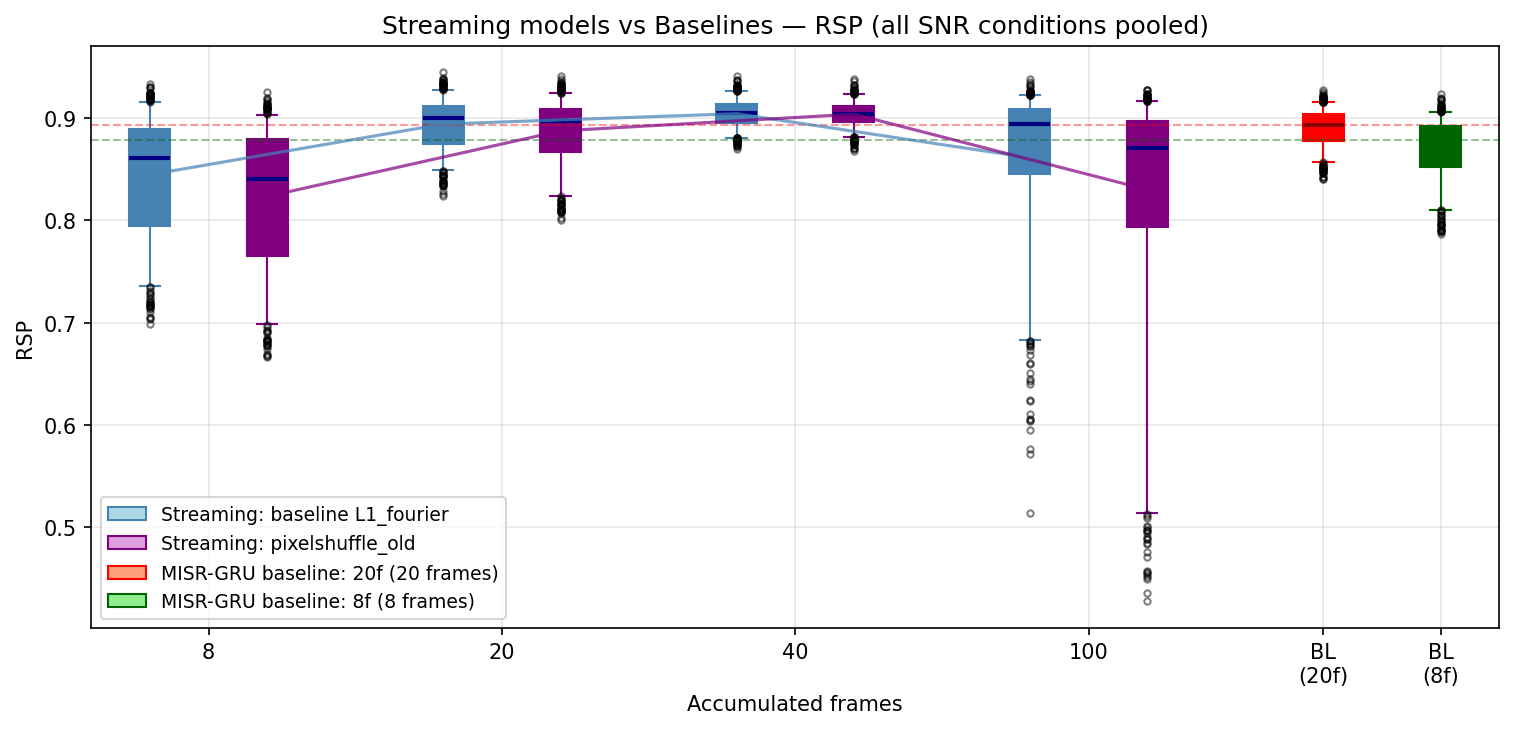
\includegraphics[width=\linewidth]{figures/streaming_pixelshuffle_vs_deconv.png}
  \caption{RSP per SNR condition for streaming MISRGRU with a PixelShuffle decoder
           versus a transposed-convolution decoder.}
  \label{fig:streaming_pixelshuffle_vs_deconv}
\end{figure}

Figure~\ref{fig:streaming_pixelshuffle_vs_deconv} shows that the transposed-convolution
decoder performs slightly better than PixelShuffle on all pooled SNR conditions.
We believe the issue comes from the croping to match $2n{-}7$ upscaling, while
transposed convolution maps directly to the exact $(2H-7)\times(2W-7)$ output grid and
avoids this issue.


